\documentclass{beamer}
\usepackage{graphicx}
\usepackage{xcolor}
\usepackage{tikz}
\usepackage{fontawesome5}
\usepackage{hyperref}
\usepackage{listings}
\usepackage{amsfonts}
\usetikzlibrary{shapes,arrows,positioning,fit,calc,backgrounds,decorations.markings,patterns}

\usetheme{RedHat}

%% Set the logo
\redhatlogo{redhat-logo.png}

%% Color definitions
\definecolor{accentblue}{RGB}{50,100,180}
\definecolor{accentgreen}{RGB}{40,167,69}
\definecolor{accentorange}{RGB}{230,150,30}
\definecolor{accentred}{RGB}{220,53,69}
\definecolor{accentpurple}{RGB}{120,60,180}
\definecolor{accentgray}{RGB}{100,100,100}
\definecolor{lightbg}{RGB}{240,242,245}
\definecolor{codepurple}{rgb}{0.58,0,0.82}
\definecolor{codegreen}{rgb}{0,0.6,0}
\definecolor{codegray}{rgb}{0.5,0.5,0.5}
\definecolor{backcolour}{rgb}{0.95,0.95,0.92}
\definecolor{cardwhite}{RGB}{255,255,255}
\definecolor{dashbg}{RGB}{240,242,245}
\definecolor{headerblue}{RGB}{40,60,100}
\definecolor{sidebarblue}{RGB}{30,50,80}

%% Code styling
\lstdefinestyle{mystyle}{
    backgroundcolor=\color{backcolour},
    basicstyle=\ttfamily\tiny,
    breaklines=true,
    captionpos=b,
    commentstyle=\color{codegreen},
    keywordstyle=\color{magenta},
    stringstyle=\color{codepurple},
    numberstyle=\tiny\color{codegray},
    showspaces=false,
    showtabs=false,
    tabsize=2
}
\lstdefinestyle{yamlstyle}{
    backgroundcolor=\color{lightbg},
    basicstyle=\ttfamily\tiny,
    breaklines=true,
    keywordstyle=\color{accentblue}\bfseries,
    stringstyle=\color{accentgreen},
    commentstyle=\color{accentgray},
    showstringspaces=false,
    tabsize=2
}
\lstset{style=mystyle}

%% Title Information
\title{Test Presentation}
\subtitle{Template Feature Showcase}
\author{Author Name}
\secondauthor{Second Author Name}
\date{March 25, 2026}

\slidedescription{Template Demo}

\begin{document}

%% Title Slide
\begin{frame}[plain]
  \titlepage
\end{frame}

%% Index Slide
\begin{frame}{Index}
  \tiny
  \tableofcontents
\end{frame}

\section{Text and Blocks}

\begin{frame}{Standard Block Types}
  \begin{block}{Information Block}
    \scriptsize
    This is a standard \textbf{block} environment used for general information.
    It supports \textit{italic}, \textbf{bold}, and \texttt{monospace} text formatting.
  \end{block}

  \vspace{0.2cm}

  \begin{exampleblock}{Example Block}
    \scriptsize
    This is an \textbf{exampleblock} environment. Use it to highlight examples,
    best practices, or positive outcomes. It typically renders with a green tint.
  \end{exampleblock}

  \vspace{0.2cm}

  \begin{alertblock}{Alert Block}
    \scriptsize
    This is an \textbf{alertblock} environment. Use it for warnings, critical
    information, or items that require immediate attention.
    \begin{itemize}
      \item Critical point one
      \item Critical point two
    \end{itemize}
  \end{alertblock}
\end{frame}

\begin{frame}{Font Sizes and Text Styling}
  \begin{block}{Available Font Sizes}
    \tiny This is \textbackslash tiny text \\
    \scriptsize This is \textbackslash scriptsize text \\
    \footnotesize This is \textbackslash footnotesize text \\
    \small This is \textbackslash small text \\
    \normalsize This is \textbackslash normalsize text \\
    \large This is \textbackslash large text \\
    \Large This is \textbackslash Large text
  \end{block}

  \vspace{0.2cm}

  \begin{exampleblock}{Dynamic Font Sizing}
    \scriptsize
    Use \texttt{\textbackslash fontsize\{size\}\{skip\}\textbackslash selectfont} for precise control: \\
    {\fontsize{6}{7}\selectfont This is fontsize 6/7} \quad
    {\fontsize{8}{9}\selectfont This is fontsize 8/9} \quad
    {\fontsize{10}{12}\selectfont This is fontsize 10/12}
  \end{exampleblock}

  \vspace{0.2cm}

  \scriptsize
  \textbf{Colored text:}
  \textcolor{accentblue}{Blue text},
  \textcolor{accentgreen}{Green text},
  \textcolor{accentred}{Red text},
  \textcolor{accentorange}{Orange text},
  \textcolor{accentpurple}{Purple text}
\end{frame}

\section{Lists and Columns}

\begin{frame}{Itemize and Enumerate Lists}
  \begin{columns}[T]
    \begin{column}{0.48\textwidth}
      \textbf{Bullet List (itemize):}
      \scriptsize
      \begin{itemize}
        \setlength{\itemsep}{3pt}
        \item First level item
        \item Another first level item
          \begin{itemize}
            \item Second level nested item
            \item Another nested item
              \begin{itemize}
                \item Third level item
              \end{itemize}
          \end{itemize}
        \item Back to first level
      \end{itemize}

      \vspace{0.2cm}

      \textbf{Compact List:}
      \begin{itemize}
        \setlength{\itemsep}{0pt}
        \item Tight spacing item one
        \item Tight spacing item two
        \item Tight spacing item three
      \end{itemize}
    \end{column}
    \begin{column}{0.48\textwidth}
      \textbf{Numbered List (enumerate):}
      \scriptsize
      \begin{enumerate}
        \setlength{\itemsep}{3pt}
        \item First numbered item
        \item Second numbered item
          \begin{enumerate}
            \item Nested numbered item
            \item Another nested item
          \end{enumerate}
        \item Third numbered item
        \item Fourth numbered item
      \end{enumerate}

      \vspace{0.2cm}

      \textbf{Mixed List:}
      \begin{enumerate}
        \setlength{\itemsep}{0pt}
        \item Numbered parent
          \begin{itemize}
            \item Bullet child
            \item Another bullet child
          \end{itemize}
        \item Another numbered parent
      \end{enumerate}
    \end{column}
  \end{columns}
\end{frame}

\begin{frame}{Multi-Column Layouts}
  \begin{columns}[T]
    \begin{column}{0.30\textwidth}
      \begin{block}{\scriptsize Column 1}
        \tiny
        This is a narrow left column with a block. Useful for sidebar-style
        content or navigation summaries.
        \begin{itemize}
          \setlength{\itemsep}{0pt}
          \item Item A
          \item Item B
          \item Item C
        \end{itemize}
      \end{block}
    \end{column}
    \begin{column}{0.35\textwidth}
      \begin{exampleblock}{\scriptsize Column 2}
        \tiny
        The middle column is slightly wider. Use different block types
        across columns to create visual variety.
        \begin{enumerate}
          \setlength{\itemsep}{0pt}
          \item Step one
          \item Step two
          \item Step three
        \end{enumerate}
      \end{exampleblock}
    \end{column}
    \begin{column}{0.30\textwidth}
      \begin{alertblock}{\scriptsize Column 3}
        \tiny
        Right column with alert styling. Great for warnings or
        important notes that complement the main content.
      \end{alertblock}

      \vspace{0.1cm}

      \begin{block}{\scriptsize Extra Block}
        \tiny
        Multiple blocks can stack vertically within a single column.
      \end{block}
    \end{column}
  \end{columns}
\end{frame}

\section{Code Snippets}

\begin{frame}[fragile]{Code Listing - Bash and Python}
  \begin{columns}[T]
    \begin{column}{0.48\textwidth}
      \begin{lstlisting}[language=bash, numbers=left, basicstyle=\ttfamily\tiny, title={\tiny\bfseries Shell Script Example}]
#!/bin/bash
# Deploy application to staging
set -euo pipefail

DEPLOY_ENV="${1:-staging}"
IMAGE="registry.example.com/app:latest"

echo "Deploying to ${DEPLOY_ENV}..."

podman pull "${IMAGE}"
podman run -d \
  --name myapp \
  -p 8080:8080 \
  -e ENV="${DEPLOY_ENV}" \
  "${IMAGE}"

echo "Deployment complete!"
      \end{lstlisting}
    \end{column}
    \begin{column}{0.48\textwidth}
      \begin{lstlisting}[language=python, numbers=left, basicstyle=\ttfamily\tiny, title={\tiny\bfseries Python Example}]
#!/usr/bin/env python3
"""Sample API client."""
import requests
from typing import Optional

class APIClient:
    def __init__(self, base_url: str):
        self.base_url = base_url
        self.session = requests.Session()

    def get_status(self) -> dict:
        """Fetch service status."""
        resp = self.session.get(
            f"{self.base_url}/api/v1/status"
        )
        resp.raise_for_status()
        return resp.json()

if __name__ == "__main__":
    client = APIClient("https://api.example.com")
    print(client.get_status())
      \end{lstlisting}
    \end{column}
  \end{columns}
\end{frame}

\begin{frame}[fragile]{Code Listing - YAML and JSON}
  \begin{columns}[T]
    \begin{column}{0.50\textwidth}
      \begin{lstlisting}[style=yamlstyle, basicstyle=\ttfamily\fontsize{4.5}{5.5}\selectfont, title={\tiny\bfseries Kubernetes Deployment (YAML)}]
apiVersion: apps/v1
kind: Deployment
metadata:
  name: my-application
  namespace: production
  labels:
    app: my-app
    version: v2.1.0
spec:
  replicas: 3
  selector:
    matchLabels:
      app: my-app
  template:
    metadata:
      labels:
        app: my-app
    spec:
      containers:
        - name: app
          image: registry.example.com/app:v2.1.0
          ports:
            - containerPort: 8080
          resources:
            limits:
              memory: "256Mi"
              cpu: "500m"
          livenessProbe:
            httpGet:
              path: /healthz
              port: 8080
            initialDelaySeconds: 10
      \end{lstlisting}
    \end{column}
    \begin{column}{0.50\textwidth}
      \begin{lstlisting}[language=, basicstyle=\ttfamily\fontsize{4.5}{5.5}\selectfont, title={\tiny\bfseries API Response (JSON)}]
{
  "status": "healthy",
  "version": "2.1.0",
  "components": {
    "database": {
      "status": "connected",
      "latency_ms": 12
    },
    "cache": {
      "status": "connected",
      "hit_rate": 0.94
    },
    "queue": {
      "status": "connected",
      "pending_jobs": 42
    }
  },
  "metrics": {
    "requests_per_sec": 1250,
    "error_rate": 0.002,
    "p99_latency_ms": 145,
    "active_connections": 89
  },
  "uptime_seconds": 864000
}
      \end{lstlisting}
    \end{column}
  \end{columns}
\end{frame}

\begin{frame}[fragile]{Code in Blocks and Verbatim}
  \begin{exampleblock}{\scriptsize Configuration Example}
    \begin{lstlisting}[language=bash, numbers=none, basicstyle=\ttfamily\fontsize{5}{6}\selectfont]
# /etc/myapp/config.conf
server_address = "0.0.0.0"
server_port = 8443
tls_enabled = true
tls_cert = "/etc/pki/tls/certs/server.pem"
tls_key = "/etc/pki/tls/private/server-key.pem"
log_level = "info"
    \end{lstlisting}
  \end{exampleblock}

  \vspace{0.05cm}

  \begin{block}{\scriptsize Verbatim Text Example}
    {\fontsize{5}{6}\selectfont
    \begin{verbatim}
$ curl --cert client.pem --key client-key.pem \
    https://server:8443/api/v1/status
{"status":"ok","version":"2.1.0"}
    \end{verbatim}}
  \end{block}

  \vspace{0.05cm}

  \begin{alertblock}{\scriptsize Important Note}
    \tiny
    Use \texttt{[fragile]} frame option when including \texttt{lstlisting} or
    \texttt{verbatim} environments. Without it, LaTeX will fail to compile.
  \end{alertblock}
\end{frame}

\section{Tables}

\begin{frame}{Basic Table with Headers}
  \begin{block}{Component Overview}
    \scriptsize
    Tables use the \texttt{tabular} environment with column specifiers:
    \texttt{l} (left), \texttt{c} (center), \texttt{r} (right), \texttt{p\{width\}} (paragraph).
  \end{block}

  \vspace{0.2cm}

  \begin{center}
    \scriptsize
    \begin{tabular}{|l|l|p{5cm}|}
      \hline
      \textbf{Layer} & \textbf{Component} & \textbf{Technology} \\
      \hline
      \hline
      Frontend & Web UI & React.js + TypeScript \\
      \hline
      Backend & API Server & Rust (Axum) + Tokio \\
      \hline
      Storage & Database & PostgreSQL / TimescaleDB \\
      \hline
      Storage & Cache & Redis \\
      \hline
      Auth & Identity & Keycloak / OIDC \\
      \hline
      Observability & Metrics & Prometheus + Grafana \\
      \hline
    \end{tabular}
  \end{center}
\end{frame}

\begin{frame}{Comparison Table with Colors}
  \begin{center}
    \tiny
    \begin{tabular}{|p{3.5cm}|c|c|c|}
      \hline
      \textbf{Metric} & \textbf{Before} & \textbf{After} & \textbf{Improvement} \\
      \hline
      \hline
      Deployment time & 45 minutes & \textbf{3 minutes} & \textcolor{accentgreen}{15x faster} \\
      \hline
      Incident detection & Hours & \textbf{Seconds} & \textcolor{accentgreen}{100x faster} \\
      \hline
      Configuration drift & Unknown & \textbf{Tracked} & \textcolor{accentgreen}{Full visibility} \\
      \hline
      Rollback capability & Manual & \textbf{Automated} & \textcolor{accentgreen}{One-click} \\
      \hline
      Test coverage & 45\% & \textbf{92\%} & \textcolor{accentgreen}{2x increase} \\
      \hline
      Mean time to recovery & 4 hours & \textbf{15 minutes} & \textcolor{accentgreen}{16x faster} \\
      \hline
    \end{tabular}
  \end{center}

  \vspace{0.3cm}

  \begin{columns}[T]
    \begin{column}{0.48\textwidth}
      \begin{center}
        \scriptsize
        \begin{tabular}{|l|l|}
          \hline
          \textbf{Method} & \textbf{Best For} \\
          \hline
          Container & Quick deploys \\
          \hline
          Kubernetes & Production \\
          \hline
          RPM & Bare-metal \\
          \hline
          Systemd & Single-node \\
          \hline
        \end{tabular}
      \end{center}
    \end{column}
    \begin{column}{0.48\textwidth}
      \begin{center}
        \scriptsize
        \begin{tabular}{|l|r|}
          \hline
          \textbf{Resource} & \textbf{Allocation} \\
          \hline
          CPU & 500m \\
          \hline
          Memory & 256Mi \\
          \hline
          Storage & 10Gi \\
          \hline
          Replicas & 3 \\
          \hline
        \end{tabular}
      \end{center}
    \end{column}
  \end{columns}
\end{frame}

\section{TikZ Diagrams}

\begin{frame}{Architecture Diagram with Pillars}
  \begin{block}{Core Message}
    \scriptsize
    TikZ enables complex architectural diagrams with styled nodes, arrows, and labels.
  \end{block}

  \vspace{0.2cm}

  \begin{center}
    \begin{tikzpicture}[scale=0.62, transform shape,
        pillar/.style={rectangle, draw, thick, rounded corners,
                       text width=2.4cm, text centered, minimum height=2.8cm, font=\tiny\bfseries},
        base/.style={rectangle, draw, thick, rounded corners, fill=accentgray!10,
                     text width=11cm, text centered, minimum height=0.8cm, font=\scriptsize\bfseries}]

      \node[pillar, fill=accentblue!15] (p1) at (0,0) {
        \faIcon{project-diagram}\\[4pt]
        Service\\Discovery\\[4pt]
        \normalfont\tiny DNS-based\\
        Health checks\\
        Load balancing
      };
      \node[pillar, fill=accentgreen!15] (p2) at (3.2,0) {
        \faDatabase\\[4pt]
        Data\\Layer\\[4pt]
        \normalfont\tiny PostgreSQL\\
        Redis cache\\
        TimescaleDB
      };
      \node[pillar, fill=accentorange!15] (p3) at (6.4,0) {
        \faIcon{chart-bar}\\[4pt]
        Observability\\[4pt]
        \normalfont\tiny OpenTelemetry\\
        Prometheus\\
        Grafana
      };
      \node[pillar, fill=accentpurple!15] (p4) at (9.6,0) {
        \faIcon{shield-alt}\\[4pt]
        Security\\[4pt]
        \normalfont\tiny mTLS\\
        RBAC\\
        Audit logging
      };

      % Base
      \node[base] (b) at (4.8,-2.4) {
        \faPlug\ \ Infrastructure Layer (Kubernetes $\cdot$ Podman $\cdot$ Systemd $\cdot$ Bare Metal)
      };

      % Connections
      \draw[->, thick, accentgray] (p1) -- (p1 |- b.north);
      \draw[->, thick, accentgray] (p2) -- (p2 |- b.north);
      \draw[->, thick, accentgray] (p3) -- (p3 |- b.north);
      \draw[->, thick, accentgray] (p4) -- (p4 |- b.north);
    \end{tikzpicture}
  \end{center}

  \begin{exampleblock}{Design Principle}
    \scriptsize
    Each pillar is independently deployable. Teams can adopt components
    incrementally based on their maturity level.
  \end{exampleblock}
\end{frame}

\begin{frame}{Network Topology Diagram}
  \begin{center}
    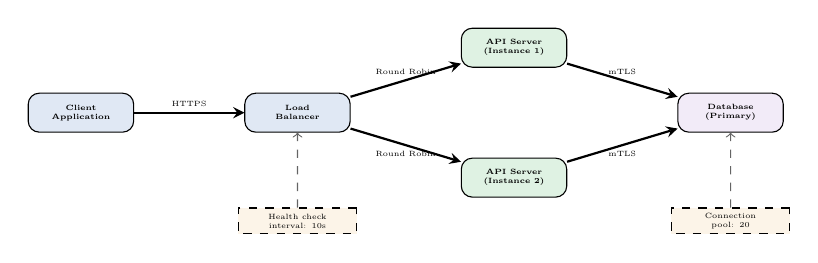
\begin{tikzpicture}[scale=0.55, transform shape,
        comp/.style={rectangle, draw, rounded corners, fill=accentblue!15, text width=2.2cm, align=center, minimum height=0.9cm, font=\tiny\bfseries},
        config/.style={rectangle, draw, dashed, fill=accentorange!10, text width=2.5cm, align=center, minimum height=0.6cm, font=\tiny},
        arrow/.style={->, >=stealth, thick}]

      \node[comp] (client) at (0,0) {Client\\Application};
      \node[comp] (lb) at (5,0) {Load\\Balancer};
      \node[comp, fill=accentgreen!15] (api1) at (10,1.5) {API Server\\(Instance 1)};
      \node[comp, fill=accentgreen!15] (api2) at (10,-1.5) {API Server\\(Instance 2)};
      \node[comp, fill=accentpurple!10] (db) at (15,0) {Database\\(Primary)};

      \node[config] (c1) at (5,-2.5) {Health check\\interval: 10s};
      \node[config] (c2) at (15,-2.5) {Connection\\pool: 20};

      \draw[arrow] (client) -- node[above, font=\tiny] {HTTPS} (lb);
      \draw[arrow] (lb) -- node[above, font=\tiny] {Round Robin} (api1);
      \draw[arrow] (lb) -- node[below, font=\tiny] {Round Robin} (api2);
      \draw[arrow] (api1) -- node[above, font=\tiny] {mTLS} (db);
      \draw[arrow] (api2) -- node[below, font=\tiny] {mTLS} (db);

      \draw[->, dashed, accentgray] (c1) -- (lb);
      \draw[->, dashed, accentgray] (c2) -- (db);
    \end{tikzpicture}
  \end{center}

  \vspace{0.2cm}

  \begin{columns}[T]
    \begin{column}{0.48\textwidth}
      \begin{block}{Network Properties}
        \scriptsize
        \begin{itemize}
          \setlength{\itemsep}{0pt}
          \item End-to-end TLS encryption
          \item Health-based routing
          \item Automatic failover
          \item Connection pooling
        \end{itemize}
      \end{block}
    \end{column}
    \begin{column}{0.48\textwidth}
      \begin{alertblock}{Security Notes}
        \scriptsize
        \begin{itemize}
          \setlength{\itemsep}{0pt}
          \item All connections use mTLS
          \item Certificate rotation every 90 days
          \item Network policies restrict access
          \item Audit logging on all endpoints
        \end{itemize}
      \end{alertblock}
    \end{column}
  \end{columns}
\end{frame}

\begin{frame}{Pie Chart and Line Graph}
  \begin{columns}[T]
    \begin{column}{0.45\textwidth}
      \begin{center}
        \textbf{\scriptsize Resource Distribution}

        \vspace{0.2cm}

        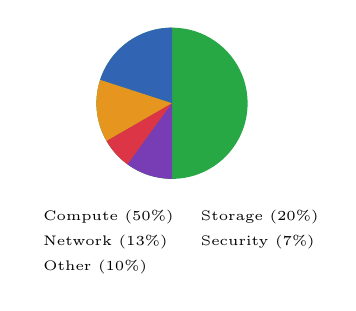
\begin{tikzpicture}[scale=0.8]
          % Pie chart (shifted right to center visually within the column)
          \fill[accentgreen] (0.8,0) circle (1.2);
          \fill[accentblue] (0.8,0) -- ++(90:1.2) arc(90:162:1.2) -- cycle;
          \fill[accentorange] (0.8,0) -- ++(162:1.2) arc(162:210:1.2) -- cycle;
          \fill[accentred] (0.8,0) -- ++(210:1.2) arc(210:234:1.2) -- cycle;
          \fill[accentpurple] (0.8,0) -- ++(234:1.2) arc(234:270:1.2) -- cycle;

          % Legend
          \node[font=\tiny, anchor=west] at (-1.5,-1.8) {\textcolor{accentgreen}{$\blacksquare$} Compute (50\%)};
          \node[font=\tiny, anchor=west] at (1.0,-1.8) {\textcolor{accentblue}{$\blacksquare$} Storage (20\%)};
          \node[font=\tiny, anchor=west] at (-1.5,-2.2) {\textcolor{accentorange}{$\blacksquare$} Network (13\%)};
          \node[font=\tiny, anchor=west] at (1.0,-2.2) {\textcolor{accentred}{$\blacksquare$} Security (7\%)};
          \node[font=\tiny, anchor=west] at (-1.5,-2.6) {\textcolor{accentpurple}{$\blacksquare$} Other (10\%)};
        \end{tikzpicture}
      \end{center}
    \end{column}
    \begin{column}{0.52\textwidth}
      \begin{center}
        \textbf{\scriptsize Request Latency Over Time (24h)}

        \vspace{0.2cm}

        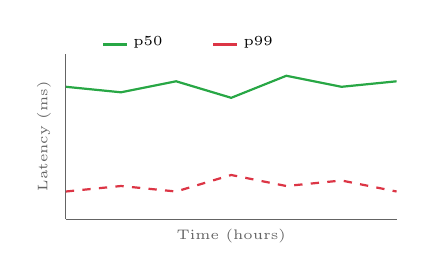
\begin{tikzpicture}[scale=0.7]
          % Axes
          \draw[accentgray, thin] (0,0) -- (0,3);
          \draw[accentgray, thin] (0,0) -- (6,0);

          % Simulated line chart
          \draw[accentgreen, thick] (0,2.4) -- (1,2.3) -- (2,2.5) -- (3,2.2) -- (4,2.6) -- (5,2.4) -- (6,2.5);
          \draw[accentred, thick, dashed] (0,0.5) -- (1,0.6) -- (2,0.5) -- (3,0.8) -- (4,0.6) -- (5,0.7) -- (6,0.5);

          % Labels
          \node[font=\tiny, accentgray, rotate=90] at (-0.4,1.5) {Latency (ms)};
          \node[font=\tiny, accentgray] at (3,-0.3) {Time (hours)};
          \node[font=\tiny, anchor=west] at (0.5,3.2) {\textcolor{accentgreen}{\rule{0.3cm}{1pt}} p50};
          \node[font=\tiny, anchor=west] at (2.5,3.2) {\textcolor{accentred}{\rule{0.3cm}{1pt}} p99};
        \end{tikzpicture}
      \end{center}
    \end{column}
  \end{columns}
\end{frame}

\section{Dashboard Wireframe}

\begin{frame}{Dashboard - Main Screen Layout}
  \begin{center}
    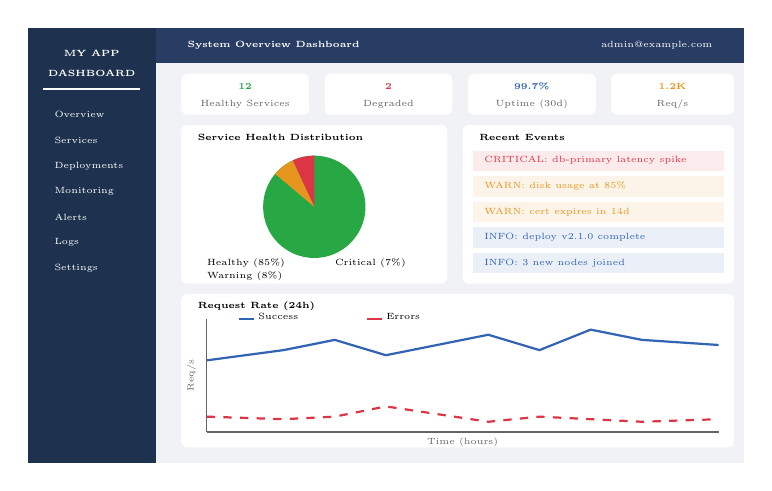
\begin{tikzpicture}[scale=0.65, transform shape]
      % Background
      \fill[dashbg] (0,0) rectangle (14,8.5);

      % Sidebar
      \fill[sidebarblue] (0,0) rectangle (2.5,8.5);
      \node[text=white, font=\tiny\bfseries] at (1.25,8) {MY APP};
      \node[text=white, font=\tiny\bfseries] at (1.25,7.6) {DASHBOARD};
      \draw[white, thick] (0.3,7.3) -- (2.2,7.3);

      % Sidebar menu items
      \foreach \y/\label in {6.8/Overview, 6.3/Services, 5.8/Deployments, 5.3/Monitoring, 4.8/Alerts, 4.3/Logs, 3.8/Settings} {
        \node[text=white!80, font=\tiny, anchor=west] at (0.4,\y) {\label};
      }

      % Header bar
      \fill[headerblue] (2.5,7.8) rectangle (14,8.5);
      \node[text=white, font=\tiny\bfseries, anchor=west] at (3,8.15) {System Overview Dashboard};
      \node[text=white!80, font=\tiny, anchor=east] at (13.5,8.15) {admin@example.com};

      % KPI Cards Row
      \fill[cardwhite, rounded corners=2pt] (3,6.8) rectangle (5.5,7.6);
      \node[font=\tiny\bfseries, accentgreen] at (4.25,7.35) {12};
      \node[font=\tiny, accentgray] at (4.25,7.0) {Healthy Services};

      \fill[cardwhite, rounded corners=2pt] (5.8,6.8) rectangle (8.3,7.6);
      \node[font=\tiny\bfseries, accentred] at (7.05,7.35) {2};
      \node[font=\tiny, accentgray] at (7.05,7.0) {Degraded};

      \fill[cardwhite, rounded corners=2pt] (8.6,6.8) rectangle (11.1,7.6);
      \node[font=\tiny\bfseries, accentblue] at (9.85,7.35) {99.7\%};
      \node[font=\tiny, accentgray] at (9.85,7.0) {Uptime (30d)};

      \fill[cardwhite, rounded corners=2pt] (11.4,6.8) rectangle (13.8,7.6);
      \node[font=\tiny\bfseries, accentorange] at (12.6,7.35) {1.2K};
      \node[font=\tiny, accentgray] at (12.6,7.0) {Req/s};

      % Status Distribution (left chart)
      \fill[cardwhite, rounded corners=2pt] (3,3.5) rectangle (8.2,6.6);
      \node[font=\tiny\bfseries, anchor=west] at (3.2,6.35) {Service Health Distribution};
      \fill[accentgreen] (5.6,5) circle (1);
      \fill[accentred] (5.6,5) -- ++(90:1) arc(90:115:1) -- cycle;
      \fill[accentorange] (5.6,5) -- ++(115:1) arc(115:140:1) -- cycle;
      \node[font=\tiny, anchor=west] at (3.3,3.9) {\textcolor{accentgreen}{$\blacksquare$} Healthy (85\%)};
      \node[font=\tiny, anchor=west] at (5.8,3.9) {\textcolor{accentred}{$\blacksquare$} Critical (7\%)};
      \node[font=\tiny, anchor=west] at (3.3,3.65) {\textcolor{accentorange}{$\blacksquare$} Warning (8\%)};

      % Recent Events (right panel)
      \fill[cardwhite, rounded corners=2pt] (8.5,3.5) rectangle (13.8,6.6);
      \node[font=\tiny\bfseries, anchor=west] at (8.7,6.35) {Recent Events};
      \fill[accentred!10] (8.7,5.7) rectangle (13.6,6.1);
      \node[font=\tiny, accentred, anchor=west] at (8.8,5.9) {CRITICAL: db-primary latency spike};
      \fill[accentorange!10] (8.7,5.2) rectangle (13.6,5.6);
      \node[font=\tiny, accentorange, anchor=west] at (8.8,5.4) {WARN: disk usage at 85\%};
      \fill[accentorange!10] (8.7,4.7) rectangle (13.6,5.1);
      \node[font=\tiny, accentorange, anchor=west] at (8.8,4.9) {WARN: cert expires in 14d};
      \fill[accentblue!10] (8.7,4.2) rectangle (13.6,4.6);
      \node[font=\tiny, accentblue, anchor=west] at (8.8,4.4) {INFO: deploy v2.1.0 complete};
      \fill[accentblue!10] (8.7,3.7) rectangle (13.6,4.1);
      \node[font=\tiny, accentblue, anchor=west] at (8.8,3.9) {INFO: 3 new nodes joined};

      % Timeline (bottom)
      \fill[cardwhite, rounded corners=2pt] (3,0.3) rectangle (13.8,3.3);
      \node[font=\tiny\bfseries, anchor=west] at (3.2,3.05) {Request Rate (24h)};
      \draw[accentgray, thin] (3.5,0.6) -- (3.5,2.8);
      \draw[accentgray, thin] (3.5,0.6) -- (13.5,0.6);
      \draw[accentblue, thick] (3.5,2.0) -- (5,2.2) -- (6,2.4) -- (7,2.1) -- (8,2.3) -- (9,2.5) -- (10,2.2) -- (11,2.6) -- (12,2.4) -- (13.5,2.3);
      \draw[accentred, thick, dashed] (3.5,0.9) -- (5,0.85) -- (6,0.9) -- (7,1.1) -- (8,0.95) -- (9,0.8) -- (10,0.9) -- (11,0.85) -- (12,0.8) -- (13.5,0.85);
      \node[font=\tiny, accentgray, rotate=90] at (3.2,1.7) {Req/s};
      \node[font=\tiny, accentgray] at (8.5,0.4) {Time (hours)};
      \node[font=\tiny, anchor=west] at (4,2.85) {\textcolor{accentblue}{\rule{0.3cm}{1pt}} Success};
      \node[font=\tiny, anchor=west] at (6.5,2.85) {\textcolor{accentred}{\rule{0.3cm}{1pt}} Errors};
    \end{tikzpicture}
  \end{center}
\end{frame}

\section{Icons, Colors, and Comparisons}

\begin{frame}{FontAwesome Icons Showcase}
  \begin{columns}[T]
    \begin{column}{0.48\textwidth}
      \begin{block}{\scriptsize Common Icons}
        \scriptsize
        \begin{itemize}
          \setlength{\itemsep}{2pt}
          \item \faIcon{project-diagram} \texttt{\textbackslash faIcon\{project-diagram\}}
          \item \faDatabase\ \texttt{\textbackslash faDatabase}
          \item \faIcon{chart-bar} \texttt{\textbackslash faIcon\{chart-bar\}}
          \item \faIcon{shield-alt} \texttt{\textbackslash faIcon\{shield-alt\}}
          \item \faIcon{exchange-alt} \texttt{\textbackslash faIcon\{exchange-alt\}}
          \item \faPlug\ \texttt{\textbackslash faPlug}
          \item \faTerminal\ \texttt{\textbackslash faTerminal}
          \item \faSearch\ \texttt{\textbackslash faSearch}
        \end{itemize}
      \end{block}
    \end{column}
    \begin{column}{0.48\textwidth}
      \begin{block}{\scriptsize Status Icons}
        \scriptsize
        \begin{itemize}
          \setlength{\itemsep}{2pt}
          \item \faBell\ \texttt{\textbackslash faBell}
          \item \faEye\ \texttt{\textbackslash faEye}
          \item \faClock\ \texttt{\textbackslash faClock}
          \item \faIcon{check-circle} \texttt{\textbackslash faIcon\{check-circle\}}
          \item \faIcon{times-circle} \texttt{\textbackslash faIcon\{times-circle\}}
          \item \faIcon{exclamation-triangle} \texttt{\textbackslash faIcon\{exclamation-triangle\}}
          \item \faIcon{info-circle} \texttt{\textbackslash faIcon\{info-circle\}}
          \item \faIcon{cog} \texttt{\textbackslash faIcon\{cog\}}
        \end{itemize}
      \end{block}
    \end{column}
  \end{columns}
\end{frame}

\begin{frame}{Before / After Comparison (TikZ)}
  \begin{center}
    \begin{tikzpicture}[scale=0.72, transform shape]

      % Before column
      \node[font=\small\bfseries, accentred] at (3,5) {Before};
      \draw[accentred, thick] (0.5,4.7) -- (5.5,4.7);

      \node[rectangle, draw, rounded corners, fill=accentred!8, text width=4.5cm,
            minimum height=0.7cm, font=\scriptsize, inner sep=0.15cm, anchor=west] at (0.5,4) {
        \faTerminal~Manual CLI operations
      };
      \node[rectangle, draw, rounded corners, fill=accentred!8, text width=4.5cm,
            minimum height=0.7cm, font=\scriptsize, inner sep=0.15cm, anchor=west] at (0.5,3) {
        \faSearch~Parse logs to find issues
      };
      \node[rectangle, draw, rounded corners, fill=accentred!8, text width=4.5cm,
            minimum height=0.7cm, font=\scriptsize, inner sep=0.15cm, anchor=west] at (0.5,2) {
        \faIcon{dice}~Deploy without testing
      };
      \node[rectangle, draw, rounded corners, fill=accentred!8, text width=4.5cm,
            minimum height=0.7cm, font=\scriptsize, inner sep=0.15cm, anchor=west] at (0.5,1) {
        \faIcon{bomb}~Discover issues at 3 AM
      };
      \node[rectangle, draw, rounded corners, fill=accentred!8, text width=4.5cm,
            minimum height=0.7cm, font=\scriptsize, inner sep=0.15cm, anchor=west] at (0.5,0) {
        \faIcon{file-alt}~Spend days on reports
      };

      % Arrow
      \draw[->, >=stealth, very thick, accentblue] (6,2.5) -- (7.5,2.5);

      % After column
      \node[font=\small\bfseries, accentgreen] at (11,5) {After};
      \draw[accentgreen, thick] (8.5,4.7) -- (13.5,4.7);

      \node[rectangle, draw, rounded corners, fill=accentgreen!10, text width=4.5cm,
            minimum height=0.7cm, font=\scriptsize, inner sep=0.15cm, anchor=west] at (8.5,4) {
        \faEye~Full visibility at a glance
      };
      \node[rectangle, draw, rounded corners, fill=accentgreen!10, text width=4.5cm,
            minimum height=0.7cm, font=\scriptsize, inner sep=0.15cm, anchor=west] at (8.5,3) {
        \faBell~Instant alert notifications
      };
      \node[rectangle, draw, rounded corners, fill=accentgreen!10, text width=4.5cm,
            minimum height=0.7cm, font=\scriptsize, inner sep=0.15cm, anchor=west] at (8.5,2) {
        \faIcon{check-circle}~Automated CI/CD pipeline
      };
      \node[rectangle, draw, rounded corners, fill=accentgreen!10, text width=4.5cm,
            minimum height=0.7cm, font=\scriptsize, inner sep=0.15cm, anchor=west] at (8.5,1) {
        \faClock~Proactive monitoring 24/7
      };
      \node[rectangle, draw, rounded corners, fill=accentgreen!10, text width=4.5cm,
            minimum height=0.7cm, font=\scriptsize, inner sep=0.15cm, anchor=west] at (8.5,0) {
        \faIcon{mouse-pointer}~One-click report generation
      };
    \end{tikzpicture}
  \end{center}
\end{frame}

\begin{frame}{\fontsize{11}{13}\selectfont Color Palette and Mathematical Symbols}
  \begin{columns}[T]
    \begin{column}{0.48\textwidth}
      \begin{block}{\scriptsize Defined Color Palette}
        \scriptsize
        \begin{tabular}{|l|l|}
          \hline
          \textbf{Name} & \textbf{Preview} \\
          \hline
          accentblue & \textcolor{accentblue}{$\blacksquare\blacksquare\blacksquare$} \\
          \hline
          accentgreen & \textcolor{accentgreen}{$\blacksquare\blacksquare\blacksquare$} \\
          \hline
          accentorange & \textcolor{accentorange}{$\blacksquare\blacksquare\blacksquare$} \\
          \hline
          accentred & \textcolor{accentred}{$\blacksquare\blacksquare\blacksquare$} \\
          \hline
          accentpurple & \textcolor{accentpurple}{$\blacksquare\blacksquare\blacksquare$} \\
          \hline
          accentgray & \textcolor{accentgray}{$\blacksquare\blacksquare\blacksquare$} \\
          \hline
        \end{tabular}
      \end{block}
    \end{column}
    \begin{column}{0.48\textwidth}
      \begin{block}{\scriptsize Mathematical Symbols}
        \scriptsize
        \begin{itemize}
          \setlength{\itemsep}{2pt}
          \item Latency $\leq$ 100ms target
          \item Error rate $\approx$ 0.1\%
          \item Throughput $\geq$ 1000 req/s
          \item Cost $\sim$\$50K/year
          \item Uptime: 99.99\% ($\times$ 4 nines)
          \item Capacity: $n \times 2$ scaling
          \item $\blacktriangleright$ Bullet alternative
          \item $\bullet$ Standard bullet
        \end{itemize}
      \end{block}
    \end{column}
  \end{columns}
\end{frame}

\section{Closing}

\begin{frame}{Summary and Links}
  \begin{block}{What This Template Covers}
    \tiny
    This test presentation demonstrates all major formatting features available
    in the Red Hat Beamer theme, including:
  \end{block}

  \vspace{0.05cm}

  \tiny
  \begin{columns}[T]
    \begin{column}{0.48\textwidth}
      \begin{enumerate}
        \setlength{\itemsep}{0pt}
        \item Text blocks (block, exampleblock, alertblock)
        \item Font sizes and text styling
        \item Colored text
        \item Itemize and enumerate lists
        \item Multi-column layouts (2 and 3 columns)
        \item Code listings (bash, python, YAML, JSON)
        \item Verbatim text
      \end{enumerate}
    \end{column}
    \begin{column}{0.48\textwidth}
      \begin{enumerate}
        \setcounter{enumi}{7}
        \setlength{\itemsep}{0pt}
        \item Tables with various column types
        \item Comparison tables with color coding
        \item TikZ architecture diagrams
        \item TikZ network topology
        \item Pie charts and line graphs
        \item Dashboard wireframes
        \item Before/After comparisons
        \item FontAwesome icons
      \end{enumerate}
    \end{column}
  \end{columns}

  \vspace{0.05cm}

  \begin{exampleblock}{Useful Links}
    \tiny
    \begin{itemize}
      \setlength{\itemsep}{0pt}
      \item Repository: \url{https://github.com/sarroutbi/presentations-template}
      \item Beamer documentation: \url{https://ctan.org/pkg/beamer}
      \item TikZ/PGF manual: \url{https://ctan.org/pkg/pgf}
      \item FontAwesome5: \url{https://ctan.org/pkg/fontawesome5}
    \end{itemize}
  \end{exampleblock}
\end{frame}

\finalframe[Thank You!]


\end{document}
